\documentclass[10pt]{book}
\usepackage{mynotebook}
\usepackage{mysoftware_style}
\newcommand{\autoDir}{/Users/StupidRobot/Projects/DNP_Multiple_Frequency/notebook/auto_figures/}

\title{AWG Instrument Development}
\date{\today}
\begin{document}
\maketitle

\chapter{AWG Upgrades: Notes, Useful Ideas, and Implementation}
\section{AWG Detection Train}
\subsection{List of Necessary Improvements}
\begin{enumerate}
    \item $\Box$ Order DC - 1 GHz video amplifiers for use. Follow up with Ilia where these are actually from. 
    \item $\Box$ Measure the recovery time of the limiter.
    \item $\Box$ Get a quote and order the limiter the Kurt Warnake uses in his spectrometer. Found that the site claims 10 - 20 ns recovery of the limiters this is good however they're only rated to 100 W pulse.
    \item $\Box$ Order 2 gigatronics power supplies model number GPD 33032.
	\item $\checkmark$ Buy the F914A switch, 10 ns rise and fall time, 80 dB isolation, 1.6 dB insertion loss. However with this switch we'll have to use a diode limiter to protect the protection switch. 
    \item $\checkmark$ Need to determine the tolerance for the switch that you actually need it might not be nearly as high as you think because much of the pulse power may just be reflected back to the pulse source due to the over coupled cavity. \o[14/07/23]{You need at least 400 W tolerance in the switch.}
    \item $\checkmark$ Follow through with general microwave about the high power tolerance switch. \o[14/07/26]{They don't have one that will suffice.}
    \item $\checkmark$ Measure insertion loss from passive components e.g. DC block, high pass filter etc. \o[14/07/26]{This is just really not necessary.}
    \item $\checkmark$ Deal with DC offset for the on carrier signals. This is possibly due to a DC offset due to the IQ mixer, here just placing a DC block after the mixer or video amplifiers may deal with this. If this does not fix the issue moving a DC block around the detection train may fix this issue. Here you want to be on carrier but off EPR resonance condition this will show oscillations in signal but also the DC offset that's seen.  \o[14/07/25]{Actually it's the DC block that is causing the baseline issue, If we want to drop the base line we'd be best to modulate the LO input to the detection mixer by something like 200 MHz then use a RF high pass filter after the mixer to drop all of the DC components from the scope voltage.}
	\item $\checkmark$ Figure out what's up the weird base line after a given pulse. \o[07/24/14]{This seems to be a problem with the video amplifier bandwidth causing these distortions. You still need to go forward and measure what this is like at high power 1 W and what the base line does with changing the pulse phase and AWG frequency relative to the carrier.}
	\item $\Box$ Talk to Tim about the sensitivity measurement that Thorsten was talking about, this would be a nice experiment to do to compare our detection train to what Bruker gets.
	\item $\Box$ The phase roll and I Q imbalance of the detector is still an issue you can see it in your background traces of the ELDOR type experiment. This needs dealt with. I think if you did the calibration where you find the IQ imbalance as a function of phase and then just normalized the I and Q channels, this should at least give you a nice flat background.
\end{enumerate}
\subsection{Follow up on baseline issue 07/25/14}
I check and see that with the video amplifiers I still see this weird baseline artifact. I think that it may either be due to the band width of the amplifier or possibly due to the fact that the amplifiers reflect anything that they do not amplify. Here verify that you see the same weirdness with the DC block, then insert an isolator between the DC block and the IQ mixer to see if that fixes the issue. \o[400pm]{I do see very similar weirdness with the DC block inserted, now you should place an isolator between the DC blocks and the mixer.}
\o[442 pm]{I place the isolators in line between the IQ mixer and the DC block and see that the baseline artifact remains.}
\o[450pm]{I turn the DC block around and see the same issue. I really do think this is a band pass thing. Next take DC blocks out capture nice baseline, ft and drop anything below 50 kHz ift and see if you see a weird baseline. Interesting to note, the DC blocks do indeed drop the DC component of the spectrum.}
\o[500 pm]{I try using data analysis to show that I'm running into a bandwidth thing but find that if I drop 100 kHz I don't see any change in the spectrum. This would suggest that what I'm seeing is not a bandwidth issue but something else.}

{\bf Impedance matching?} 
\o[520 pm]{I take a 150 MHz bandpass filter and see that it removes the baseline artifact where as the DC block is actually the cause of the baseline artifact. Is it possible there is some weird impedance mismatch? I also try the 500 MHz bandpass and see that it completely removes any signal as well as the baseline artifact. This cannot be a bandpass thing.}

\o[540 pm]{I try the nicer video amplifiers and I get the same baseline artifact. What is this? I put a 150 MHz bandpass filter after the video amplifier and I see all of the baseline artifact go away. I think what you need is a highly flat amplification across the frequency range of interest. I also notice that attenuating before the video amplifier does nothing.}

I really really think that this is a problem with the video amplifier flatness. What I mean is the flatness across all frequencies being amplified.

Explanation: The DC offset comes from the IQ mixer, this is why a DC block before the mixer at XBand does nothing. The baseline drift is because we're not attenuating enough of a bandwidth, this is why with the DC block you see funky baseline but with the 150 MHz HP filter you see absolutely flat baseline. With the video amplifier you are 0.05 - 500 MHz this is cause the baseline weirdness because you aren't amplifying all frequencies equally, here you could get a really nice flat amplifier or just use a high pass filter that bocks sufficient frequencies and just make sure your signal never is in that frequency range.
Here you should buy different high pass filters and test them on the system from a look at minicircuits it looks like the lowest possible is 20 MHz which is ok but with this solution you should go with higher bandwidth video amplifiers.

\subsection{Determine the necessary tolerance for the switch 07/23/14}
Here I want to use the solid state amplifier and measure the power reflected from the resonator to the detector on the sampling scope. I should do this for various conditions of coupling and of resonance. This will tell me the relative amount of power that is reflected at the detector.
I notice that the reflection is almost half of the voltage as the input pulse. You should measure this to get a verifiable number and do for multiple resonator resonance offsets.

\subsection{Determine what component of the detection Train is causing baseline issue 07/23/14}
The base line after a pulse of any power, even low is not! flat! it should be. Here go through component by component and check what is causing this.

I see that when I'm off resonance by 100 MHz I see that the baseline after the pulse has a slow oscillation to it.

First just figure this out by pulling out the elements that may be causing the problem.

\begin{enumerate}
	\item $\checkmark$ LNA \o[5pm]{I pull this out and see that the baseline issue is still present only to a lesser extent, likely this is just amplifying the baseline problem.}
	\item $\checkmark$ limiter \o[540 pm]{I plug directly into the sampling scope and see that there is microwave leakage, you need to be using the switch so you know what is exactly the problem. It is interesting to note that I see a sort of exponential decay on the agilent where as I see an initial ripple then a DC offset on the sampling scope. I may not see the DC offset issue on the agilent because of the video amplifiers.} \o[550pm]{With the switch I effectively kill any DC offset and on the sampling scope I really just see what looks like ring down. Plug back into the agilent and see if the baseline is still there.} \o[600 pm]{I still see weirdness with the baseline. Note that when there is no microwave power in the system there is a slight disturbance with the baseline at 2 mV.} This could still be the issue.
	\item $\checkmark$ High pass filter \o[520 pm]{This does not cause the baseline issue.}
	\item $\checkmark$ Isolator \o[530 pm]{I unplug everything and go cavity -> limiter -> mixer -> VA -> scope, I still see this base line weirdness here. It's possible that this is actually due to the limiter itself, run from the limiter to the sampling scope itself.} 	\item $\Box$ IQ mixer. Here just plug the end into the sampling scope
	\item $\checkmark$ Video Amplifiers \o[610 pm]{I go cavity -> limiter -> mixer -> scope and leave out the video amplifiers, the baseline issue crap is gone or seemingly at least. Put the LNA back in place to see if that gets more power to the scope.} \o[620 pm]{I put all of the detection stuff back in and see that all of the weird baseline stuff has gone away. I also see that the DC block we have in place does nothing to X-Band which makes sense. When I put the DC blocks in I see a weird Baseline\ldots is it possible that I'm saturating the block?}
	\item $\Box$ Video Amplifiers with high power:
	\item $\Box$ Without the video amplifiers in the detection train, change the pulse phase and also change the AWG frequency and see what this corrected baseline does with changing these parameters. Actually make a plot of the baseline DC against the AWG frequency.
	\item $\Box$ Make a plot of the 50 ns pulse with the DC block in to show that this baseline issue looks very much like a poor bandpass filtering issue.
\end{enumerate}

{\bf Video Amplifiers:}
I find that the video amps are causing some sort of baseline issue I see that with out the amplifiers I have a baseline that looks very flat as shown in \ref{fig:noVA} where as when I put the amps in place I see that the base line does some weird shit as shown in \ref{fig:VA}. You really need to verify that the issue is no longer present when using higher power at least 1 - 5 Watts.

\mbox{\begin{minipage}{0.5\linewidth}

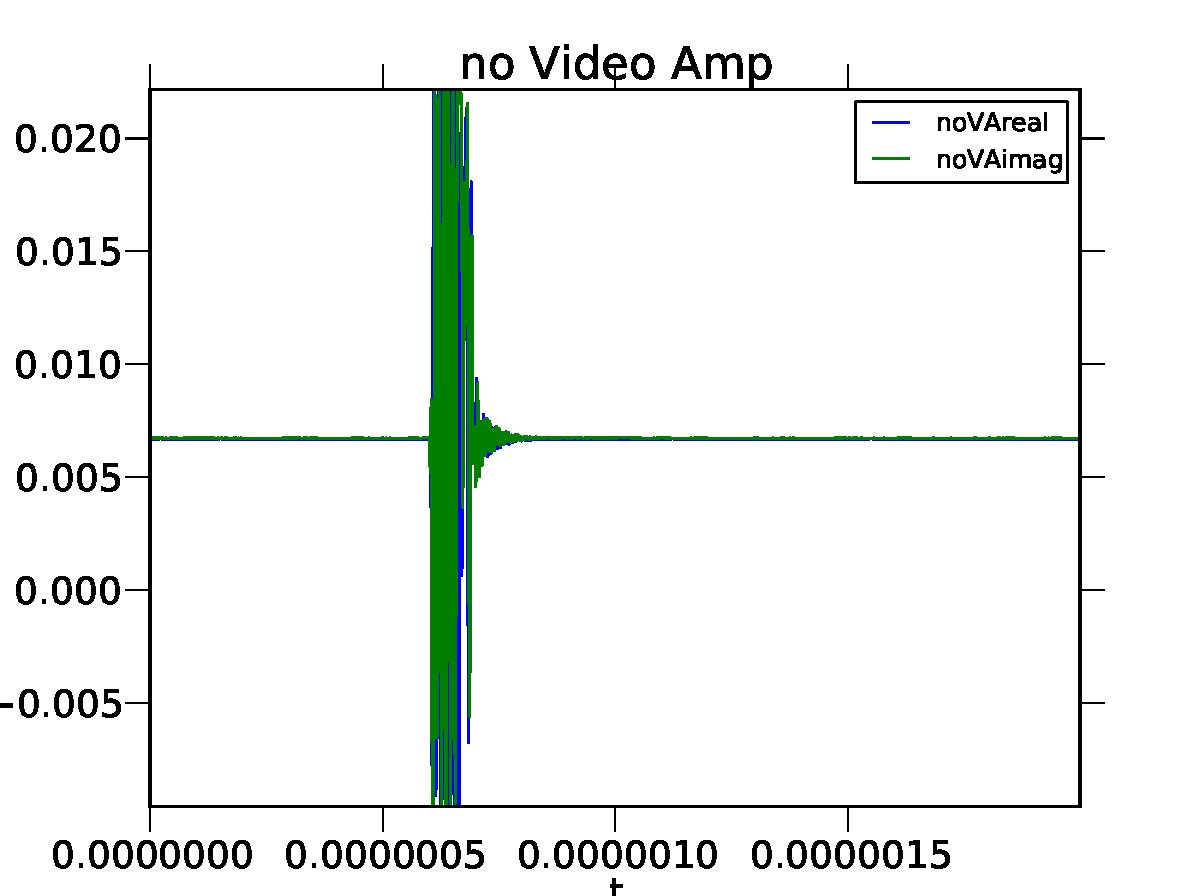
\includegraphics[width=\linewidth]{140723noVA.pdf}\label{fig:noVA}

\hrulefill 

{\color{red}{\tiny file:}:}\begin{tiny}\fn{140723noVA.pdf}\end{tiny} 

\hrulefill

\end{minipage}} \mbox{\begin{minipage}{0.5\linewidth}

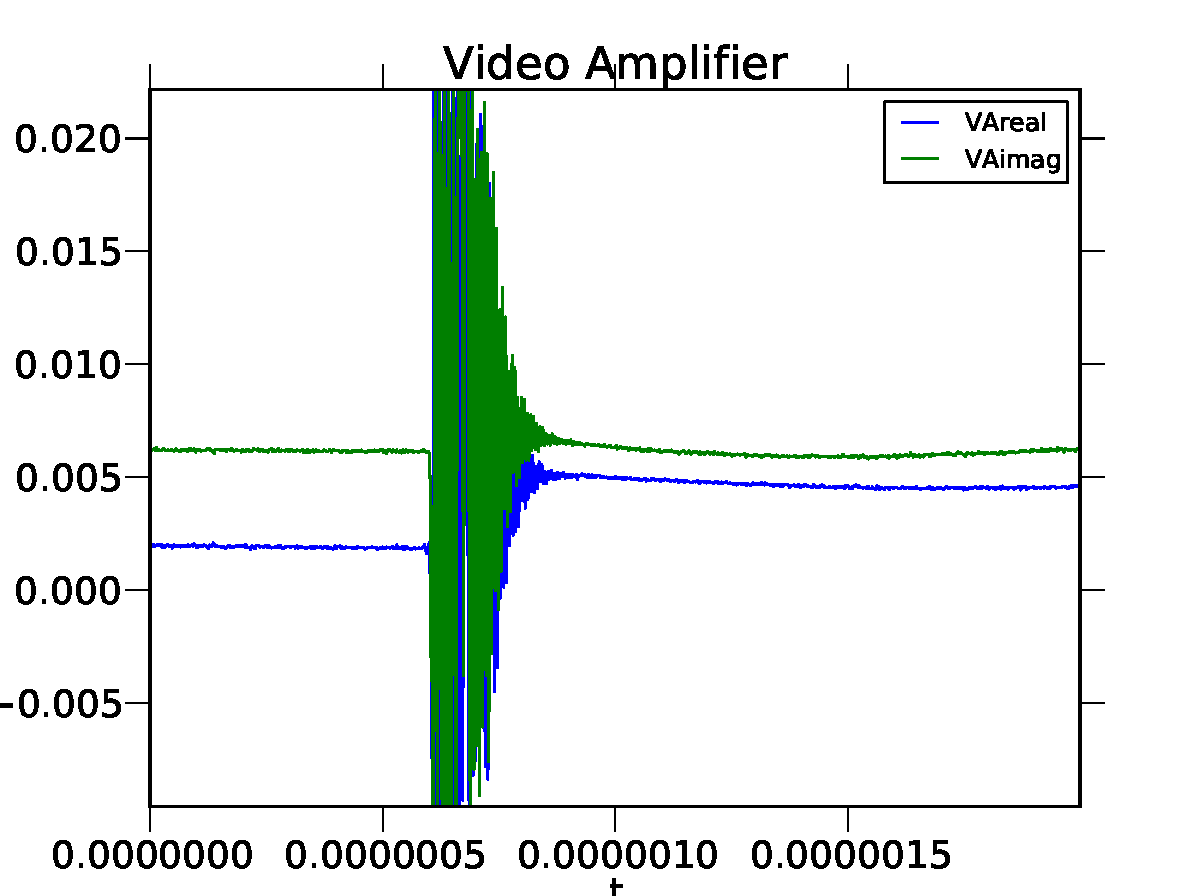
\includegraphics[width=\linewidth]{140723VA.pdf}\label{fig:VA}

\hrulefill 

{\color{red}{\tiny file:}:}\begin{tiny}\fn{140723VA.pdf}\end{tiny} 

\hrulefill

\end{minipage}}

\subsection{Implementation of 1 GHz bandwidth video amplifiers and bandpass filters}
Like the title says I implement the high bandwidth video amplifiers and the bandpass filters to deal with the baseline issue we're currently facing. \\

The figure show what we're currently dealing with. I put out a 2000 ns long pulse at low power approximately 1 mW and I see this issue.\\

\mbox{\begin{minipage}{0.5\linewidth}

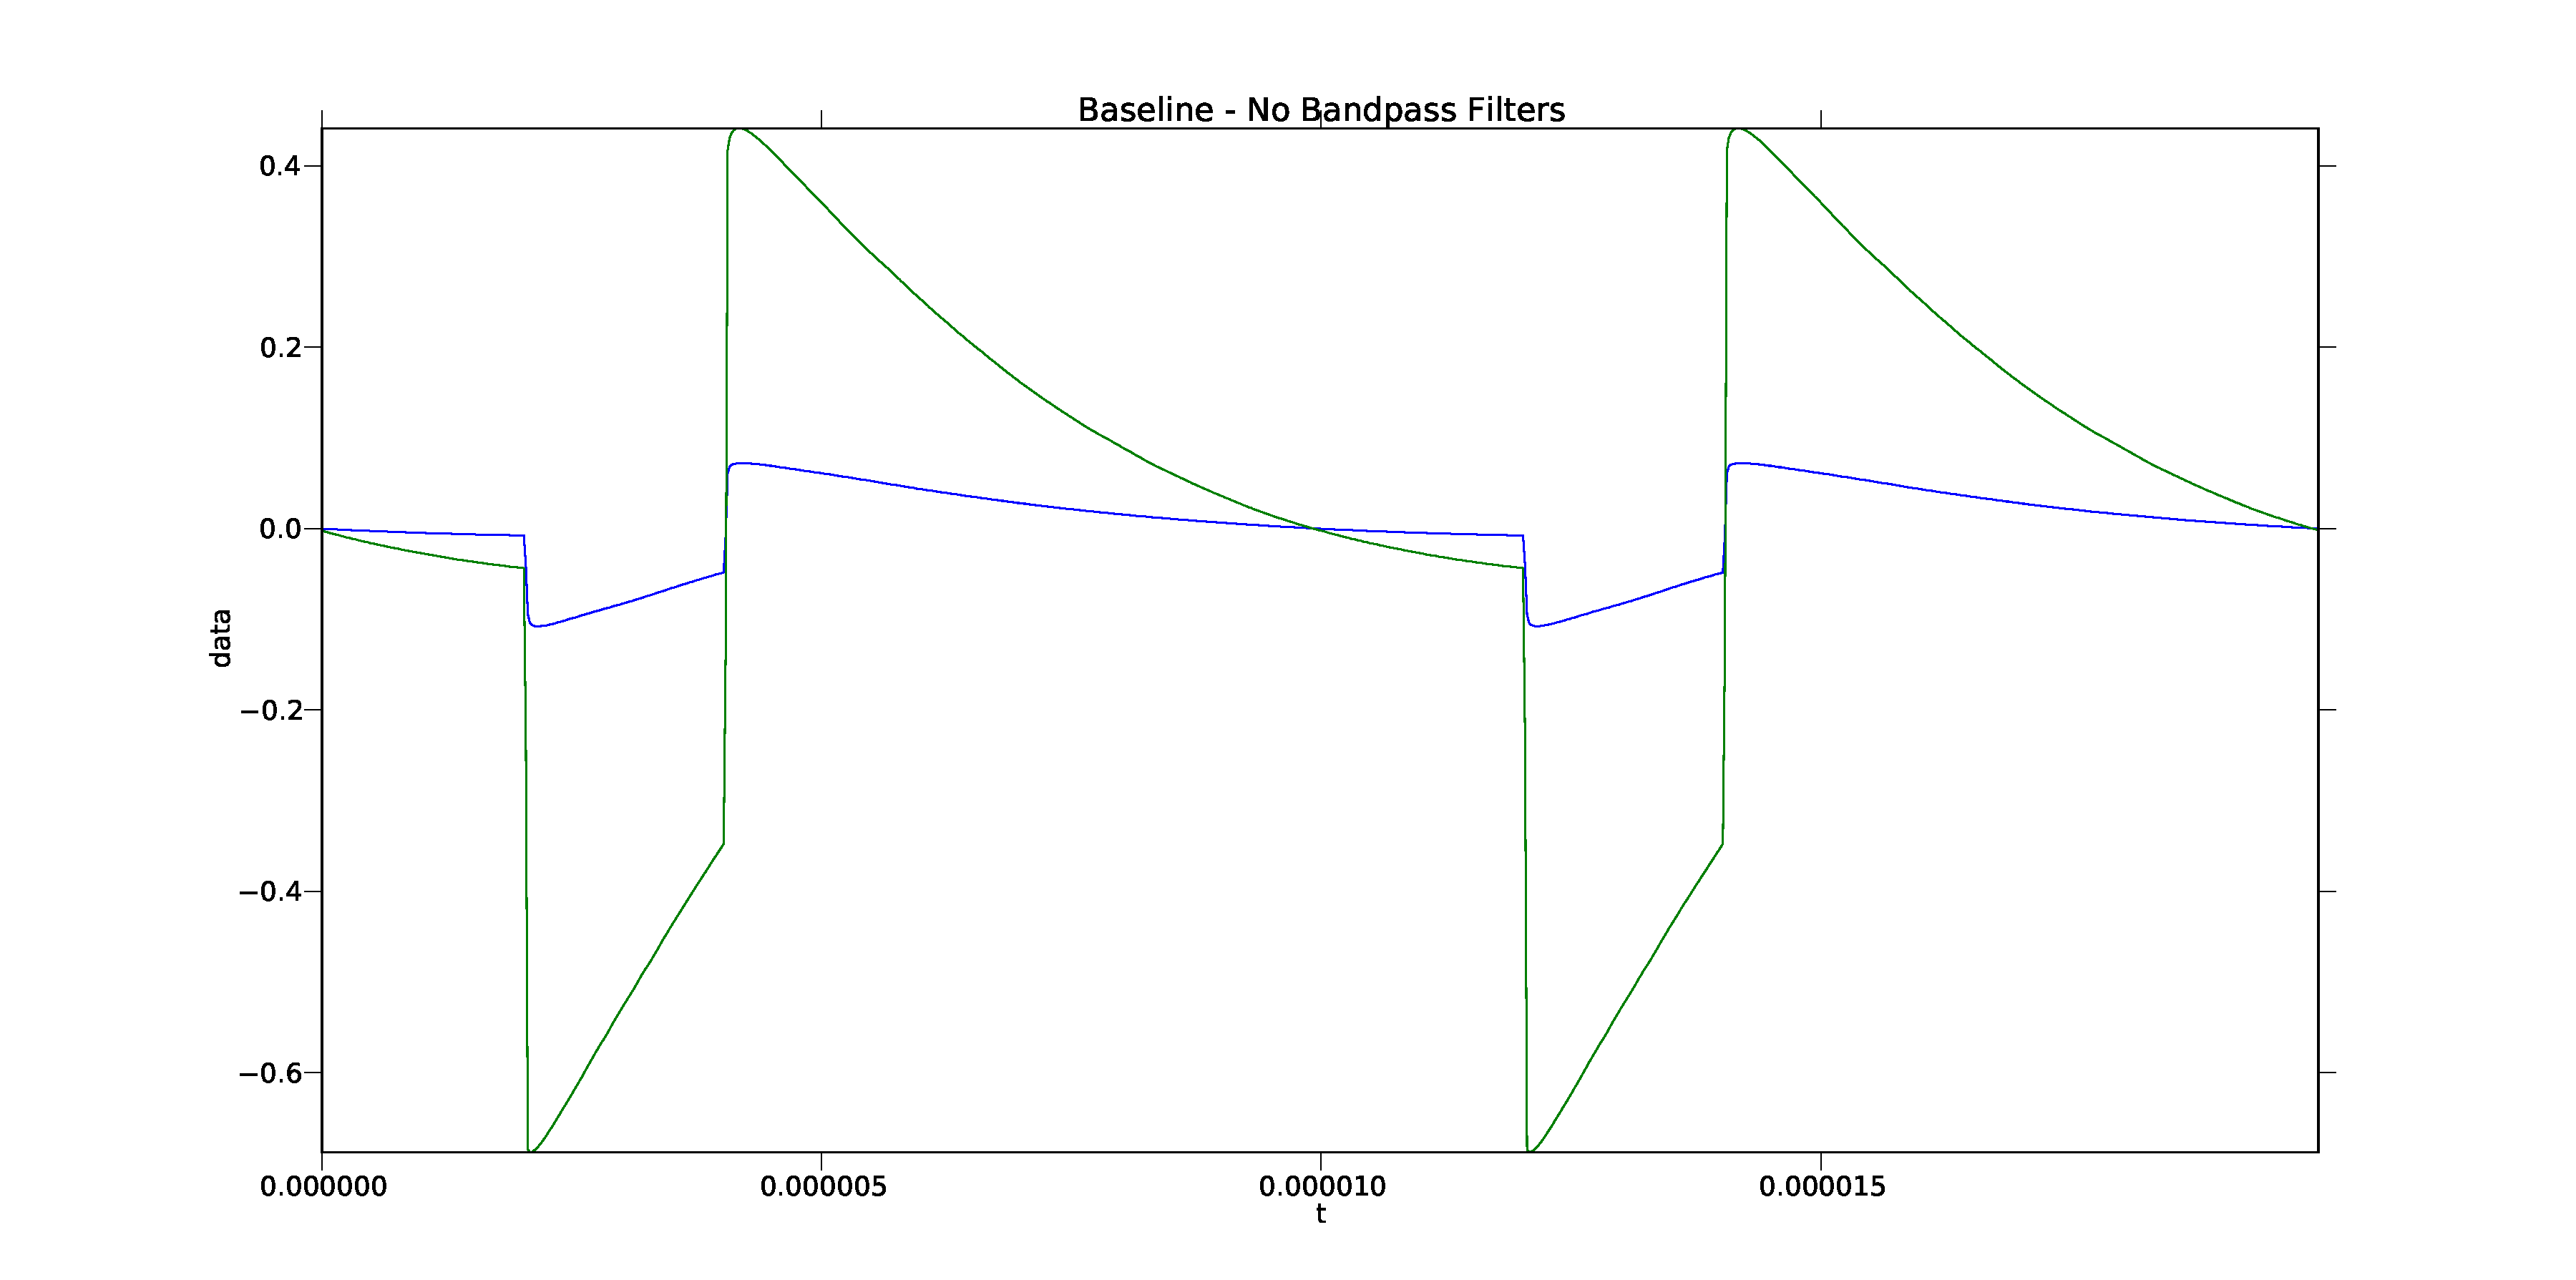
\includegraphics[width=\linewidth]{150407BAselineNoBandpass.pdf}\label{fig:noVA}

\hrulefill 

{\color{red}{\tiny file:}:}\begin{tiny}\fn{150407BAselineNoBandpass.pdf}\end{tiny} 

\hrulefill

\end{minipage}


I note that the high pass filters that I ordered from minicircuits never came in\ldots 


\subsection{Testing the reciever 15/04/09}

I setup to test the reciever with a BDPA PS sample. I tune the cavity and the

We setup with the synthesizer switch and the new reciever configuration and take some signal meausrements.


I save a representative data set as '150410Experiments.h5/phaseCycleWithBandPassWithSynthSwitch'. \o[Here we have the synthesizer switch in place and we're using the TWT. Currently the reciever switch is sitting on the shelf and not being used. I'm also using the 200 MHz bandpass filters. I set the YIG 300 MHz off resonance and use the DAC board to modulate the frequency by 300 MHz. I see that this very much cleans up the base line to my signal as I take this signal with a 4 step phase cycle. The sample is solid BPDA and I'm lookin at an echo.]{}

In preparation, I pull the synthesizer switch so the waveforms have a very high offset and I see that I still record fine signal. I repeat the same measurement and save the signal as '150410Experiments.h5/phaseCycleWithBandPassWithOutSynthSwitch'.

Also note I have a script written up to do a quick phase cycle with the modulation of the carrier by the DAC board. The script name is \o['bandpassSignalTest.py'.]{}

\section{AWG Synthesizer}
\begin{enumerate}
	\item $\Box$ Place low power (roughly 10 - 100 mW) switch and isolator after the IQ mixer to kill any leakage.
	\item $\Box$ Possibly use a phase shifter and variable attenuator 
\end{enumerate}

\subsection{Testing the Synthesizer Switch 15/04/09}

I place the switch from miteq in the synthesizer train and test to find the best configuration possible.

I find the following 
\begin{enumerate}
    \item The switch puts out a video transient at MHz frequencies when the switch turns both on and off. \o[This is why the high pass filter is in place and is bloody necessary!]{USE IT}
    \item The performance of the switch is better before the low noise amplifier as evidenced by the graph below.
    \item The input line to the switch is not impedence matched to 50 ohms. I placed a 50 ohm load to ground on the sma input and this cleans up the switch transient that is imprinted on the microwave waveform.
\end{enumerate}


I think this issue is wraped up for the moment as we have very high isolation after the pulse.

Below shows the comparison of the synthesizer switch placed before and after the input amplifier. What I find is that I get better isolation if I place the switch before the amplifier, plot shown below. \o[The Data for the plot is saved in '150409Experiments.h5']{}

Also note that this is taken without doing any zero calibration on the DAC board.

\mbox{\begin{minipage}{0.7\linewidth}

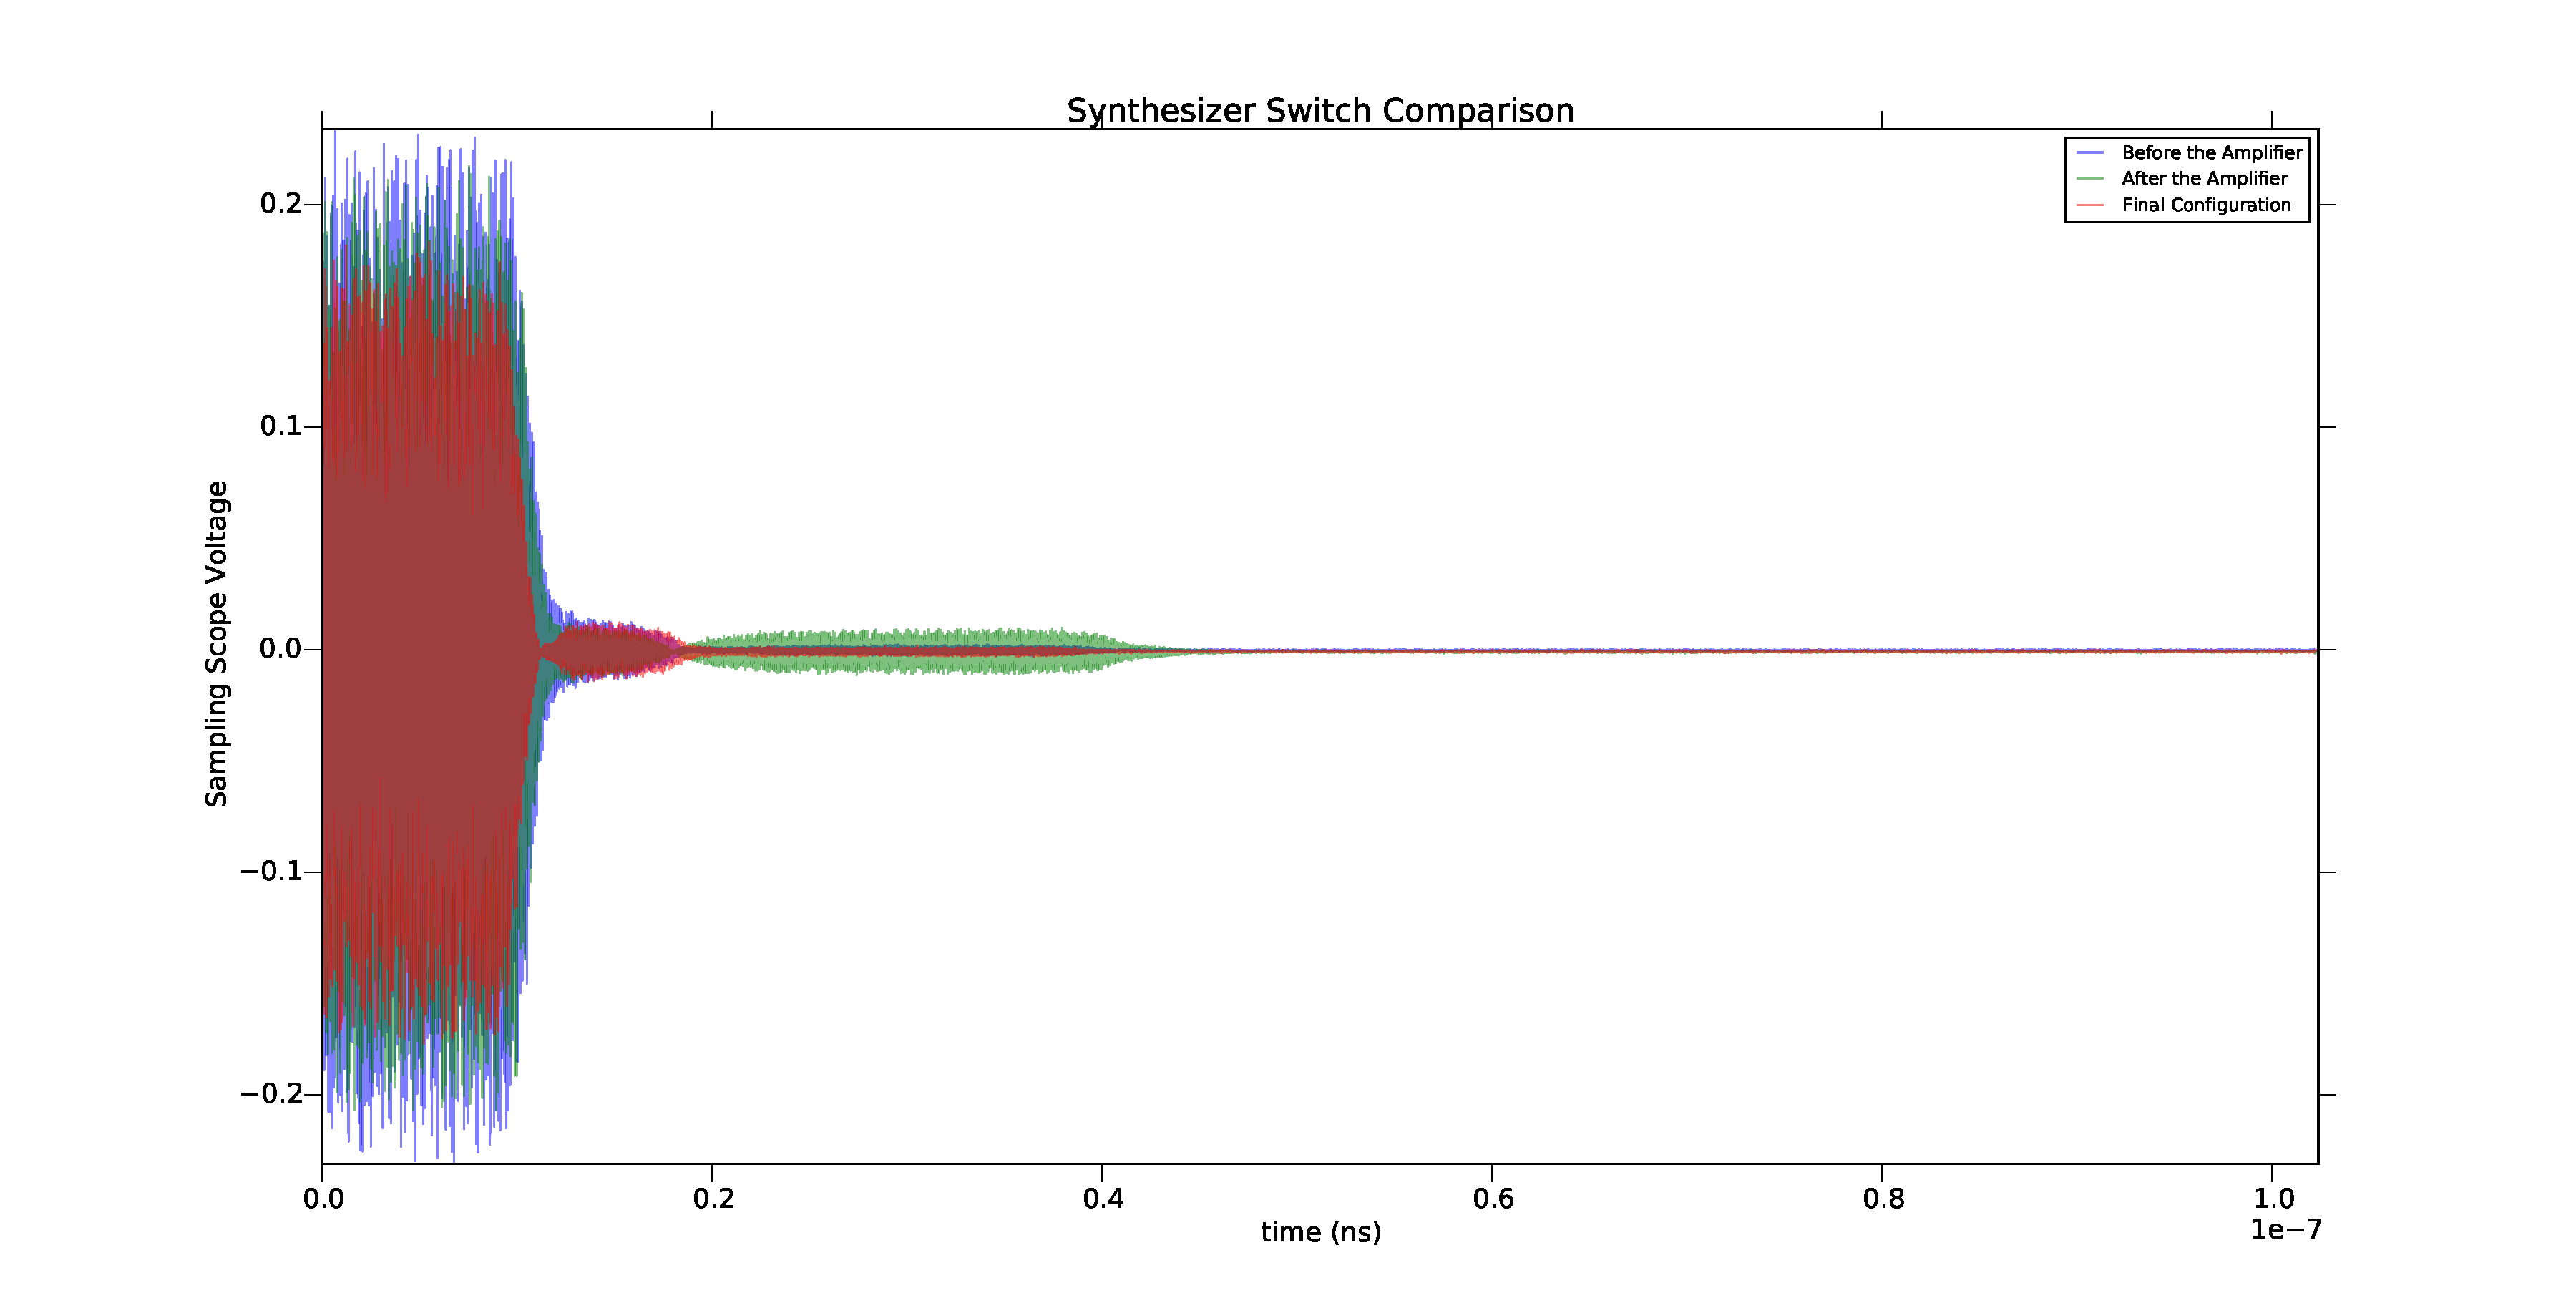
\includegraphics[width=\linewidth]{150409SynthesizerSwitchComparison.pdf}\label{fig:noVA}

\hrulefill 

{\color{red}{\tiny file:}:}\begin{tiny}\fn{150409SynthesizerSwitchComparison.pdf}\end{tiny} 

\hrulefill

\end{minipage}} 



\section{Bruker Bridge}

\chapter{DAC Board}
\section{Implementation of Daniel's new FPGA code and server software}
Daniel Sank and the Martinis group have developed some new FPGA firmware and server software to run longer pulse programs and also possibly run on board phase cycling.

\section{Time Line of Jump Tables Implementation}

I honestly think the best, most efficient, way to do this is in context of CPMG as opposed to writing nice software to handle general instances. Here I write code pragmatically to do my CPMG experiments and learn the in's and out's of using the jumptables firm ware. Once I have a handle on the firmware, I will then sit down to write code (pulsegen Class) to act as a more general implementation. At this point it would be good to get in contact with Bryan from Jayich's lab and share our code. \\

{\bf Monday (15/03/09):}
\begin{enumerate}
    \item $\checkmark$ Work with Daniel, get DAC and server program to work together. \o[Here ask Daniel the best way to do looping, imagine a CPMG sequence where you want to increment the interpulse delay, how would the jumptables vector look?]{The DAC and the server talk now. The fix was ultimately in the registry dictionary, to do with the board's fifo buffer size\ldots Also we've updated labrab and the direct ethernet program. The DAC still works with the current digitize class.} 
    \item $\Box$ Demonstrate \o[jumptables.py]{} working appropriately. \o[Need to install the current version of firmwave. V.11 not V.8]{}
    \item $\Box$ Save software example code with sufficient comments and notes to pick up project at a later date. \\
    \item $\Box$ Nuke py26.
\end{enumerate} 
Here I've come across, in a bad way, how poorly the files are organized on this box. Every module that we use is brought into the current working directory, this shouldn't be. We should store the necessary modules pulsegen, matlablike, etc. in a directory that is on the PYTHONPATH environment variable. This directory should stay clean and script that's nicely wrapped should go here and that's it!! PERIOD!!

Also you need to go through and nuke py26 and anycalls that your win scripts make to py26!! \\ \\

{\bf 3 days: Organize or Nuke Current Version of Windows\ldots Definitely NUKE IT!!}
I list thoughts below on how I think best to do this safely but this just needs done. The file organization is a mess and the computer runs like a sloth!
\begin{enumerate}
    \item $\Box$ Safely back up the HD. Detailed in {\bf This Fucking Windows Box}.
    \item $\Box$ Reformat the harddrive and re-install windows 7.
    \item $\Box$ Install all the necessary crap to make windows behave like a real development platform mingw, git, putty, python27, gcc etc.
    \item $\Box$ Copy registry keys.
    \item $\Box$ Clone pylabrad, twisted, and servers from Martinis git repo.
    \item $\Box$ Setup appropriate software directory on PYTHONPATH.
    \item $\Box$ Detail a file organization procedure so we don't end up with this mess again.
    \item $\Box$ Also set up administrator privileges to install programs, I don't really know what else to do but there is so much crap on this box.\\
\end{enumerate}


{\bf 1-3 days: Code up and test device for CPMG experiment}
\begin{enumerate}
    \item $\Box$ Use jumptabels format to produce a CPMG sequence verify all delays on scope.
    \item $\Box$ Code up a CPMG experiment where I loop through both phase of inversion pulses and the intepulse delays. \o[Do this by hand, don't attempt some fancy code structure as this will inevitably lead to a mess at this point.]{}\\
\end{enumerate}


{\bf 2-5 days: Run a CPMG experiment}
\begin{enumerate}
    \item $\Box$ Use 50\% Glycerol 4-OHT sample. cool to 85 K
    \item $\Box$ Optimize Hahn echo pulse sequence for a 200 ns interpulse spacing. Nutation
    \item $\Box$ Quickly measure a Hahn echo decay, just for the note book.
    \item $\Box$ Run a CPMG experiment with a 200 ns interpulse spacing. \o[Most likely you're going to have to do this the dumb way and use the scope to capture each echo individually, which kinda blows but it's what will be easiest. - I'm call this 'dumb-CPMG']{}\\
\end{enumerate}

Now, as proof of concept I should show the CPMG spectral filter concept. I do CPMG experiment varying the interpulse spacing and plot the decay rate $(1/T_2)$ as a function of pulse frequency.
{\bf 1 week: Spectral Filter}
\begin{enumerate}
    \item $\Box$ Measure CPMG signal as a function of pulse spacing for three different temperatures. Say 85 - 110 K, just so that I can see if what I calculate for the rotational correlation time makes sense.
    \item $\Box$ Use the $(1/T_2(\nu_{\pi}))$ data and follow Suter's method of inverting the series of equations to get my spectral density.
    \item $\Box$ Fit the spectral density to a simple lorentzian and get correlation time and plot as a function of temperature.
    \item $\Box$ Fit the spectral density to the FFHS model\\
\end{enumerate}

Here, I argue, is the right time to do instrument development (e.g. write generally implementable jump table code and configure detector to handle the CPMG experiment appropriately.) Now this is also the time to evaluate whether this is worth doing. If the Bruker setup is still orders of magnitude better in signal to noise and can also do the CPMG experiment, I argue this development is not worth doing.

If we decide it's worth doing.
{\bf 2 weeks: Code up Agilent ADC board}
\begin{enumerate}
    \item $\Box$ Demonstrate that you can capture long data packets, should be able to do $20 \mu s$ at a time with on board averaging.
    \item $\Box$ Wrap c functions to do this long data on board averaging in swig to call from python.\\
\end{enumerate}

{\bf 1 week: Wrap up jump tables into pulsegen}
\begin{enumerate}
    \item $\Box$ Write general class instance to handle parsing a given waveform into memory blocks and a list of calls for the jump tables firm ware. \o[Right now I think the easiest way is to add into the waveform class a parsing function that the user defines repeat sequences, then the class calls a function which determines from the waveform specefied and the repeat sequences the necessary list to hand jumptables so that the given waveform is reproduced.]{}\\
\end{enumerate}

\section{Jump Tables implementation}
You need to pull the data from the git hub. Pull from branch jump\_table\_bench\_test/GHzDACs

There is a readme in HanLabNewFPGA folder on desktop, it outlines what needs done.

I have the fpgaServer.py running. \o[Note that I had to comment out some code. Also on another note you might want to talk to daniel about how they organize their code.]{}

I import fpgaTest successfully and run fpgaTest.get\_build\_number(fpga,board) and cannot connect to the board because their are no fpgas present.

So far I've:
\begin{enumerate}
    \item Installed the new firmware onto the FPGA. \o[firmware located in the C:\\Users\\hanlab\\Desktop\\HanLabNewFPGAStuffs]{}
    \item Created fpgaServer from ghz\_fpga\_server.py, I had to comment out several lines that imported stuff to do with the ADC as well as imported stuff the my version of labrad does not have.
    \item Commented out lines of the fpgaTest.py for the same reasons as above. I can now import fpgaTest.py.
    \item Tried running fpgaTest.test\_jump\_table\_idle(fpga,de) \o[Here I don't know what de is I handed it cxn but I'm not sure that's what was needed.]{I also note that the mac address for the board is hard coded - I need to input the correct mac address for board.}
    \item Tried running fpga.select\_device() as well as fpga.select\_device('Han Lab DAC 1') which is the board name and I get an error telling me that no devices are present.
    \item I note that our previous method of using the startup dac board script works to bringup the DAC with the new FPGA firmware. \o[Maybe I can use this to figure out how to configure the new FPGA server program.]{I test and find the problem is isolated to the new FPGA server program. I test and use the old server program and see that I can run bringup, I close the old server and open the new one and cannot run bringup because it cannot find the DAC, I close new server open old server and run bringup successfully.}
    \item I test the dependent modules, dac.py and util.py and get the same error that bringup cannot find any board. I try moving the working server program such that it uses the new modules and see that it does not work, suggesting the new modules dac.py or util.py are to blame.
\end{enumerate}


Things I need to do:
\begin{enumerate}
    \item $\Box$ Find the correct mac address for the board and insert it, either hardcoded or as a global variable in the fpgaTest.py
    \item $\Box$ Possibly install the new labrad server.
    \item $\Box$ Talk to Daniel about file organization. There seems to be some structure you're missing that might make life easier in the long run.
      
\end{enumerate}

\section{15/02/18 - Get the board fucking working}
For some reason I can no longer connect to the DAC board. I keep getting an error when I try to connect to the DAC board \o[FAILURE: The board was off when you started the GHz DAC server. Turn on (and) connect the DAC board, close and restart the DAC server and press any key\ldots ]{}

Also, eventhough this is running on the local host loop back address this DAC server throws the same error with or without the putty ssh tunnels up and running.

I check to see that I can connect to other instruments. \o[I can connect the agilent scope, which is also setup on the loopback address. However I cannot connect the sampling scope, or more formally the prologix gpib-eth controller (setup on loopback) which is a problem in and of itself, fuck.]{}

I find that the 10 MHz oscillator is unplugged, thus the DAC is not recieving a clock signal (most likely not able to communicate because of the lack of clock signal). I plug in the clock, let it warm up, and retry connecting. What do you know, I can connect to the DAC board!!

I now try to use the DAC board, and I can synthesize waveforms good news.

The ecl port is j24 you idiot!

\section{We're in a rush to do things as always\ldots Flash the old firmware and switch back to using the old server program.}

I flash the old firmware back onto the board and setup with the old server program and things work.

I make sure to flash the .pof file because we need to be able to restart the board.

I flash the old firm ware and switch to what I think is an old version of labrad. The problem is the server program does not like when I do a long delay\ldots

Specifically I cannot run functions '\_sendDAC()' and 'fpga.run\_sequence()' with the current build, server program, and labrad implemnetation. 

I need to fix this as we need to be able to run sequences longer than $15 \mu s$. The things I try are below.
\begin{enumerate}
    \item $\checkmark$ Try updating to the new version of the labrad. \o[This didn't work for allowing the use of sending and playing memory]{Balls}
    \item $\checkmark$ Try loading the old labrad in site_packages. \o[Again this didn't work]{}
    \item $\checkmark$ Try the old server progam and make sure it's using the old labrad version. \o[Yes, using old version of labrad and the old server. Still Didn't work]{}
    \item $\checkmark$ Flash what you think to be the old build onto the board, I found \o[V5_b8]{} on the Martinis website and tried that but I still get the 'Paging off: SRAM too long.' error. \o[I see the registry has definitions for the sram length that look right but I now check what length of sram I'm sending to the DAC.]{This isn't a build problem\ldots This is something to do with the server or the registry.}
    \item $\checkmark$ Check sram length, maybe this error is real and not something to do with the old server / build. \o[No it's the proper length.]{FUCK!}
    \item $\checkmark$ Do build 14. The new server. The new labrad. Daniel got back to me about the issue being resolved\ldots Maybe this will work now? \o[Make sure to test with the 'testBuild14.py', this code runs through a jump\_table example that Daniel gave me and also plays an sram sequence. Also make sure you try all build numbers. ]{I got through and try all build numbers and cannot get the board to function when sending jumptable commands.}
\end{enumerate}

\subsection{15/04/12}

Conclusion to previous day of work. Jump tables will not work at this time due to continued development at the Martinis group\ldots The problem is I need to loop over memory to do long delays which I currently cannot do. \\

{\bf Make a test script for Daniel that shows the sram and the memory I send to the DAC board. Do this running the new server and the newest version of pylabrad.}


\begin{enumerate}
    \item I'm now running the newest version of pylabrad on master branch and the newest version of servers on jump\_table\_test\_bench branch.
\end{enumerate}


\chapter{The Prologix Controller}

This does deserve it's own chapter as you spent two days figuring this out\ldots The power supply is truly important. You found that it is very important that it supply the right power, if it's not right the prologix controller will still light up and 'look' normal however it will not function properly as an tcp / ip socket.

I can now access the field controller and I setup the gpibtunnels in putty to forward or tunnel or whatever it's called through this new address. 

I can now access the gpib controller via 'conn = g.gpib()' and the field controller through 'fc = g.field\_controller()'. The new computer is still a problem but atleast this is fixed.


\chapter{This Fucking Windows Computer - Rebooting and Getting the DAC to work with New Comp and Firmware}
Seriously, it needs reformatted\ldots BADLY! 

I am hesitant to do this bing bang boom as it will be a pain in the ass to get resetup and working nicely again. I list what I think would be a good plan of action for re-formating this piece of shit.\\

{\bf Didn't go this route.}

\begin{enumerate}
    \item $\Box$ Mirror the current hard drive on an external drive.
    \item $\Box$ Verify that you can boot into this drive off of the windows box.
    \item $\Box$ Make sure you have access to pylabrad and servers repositories from the Martinis group on the github. 
    \item $\Box$ back up the registry files so that you can reconnect to the board.
    \item $\Box$ Make sure you can access quartus on the new computer, or get an access key.
    \item $\Box$ Now reformat that shit box and install a fresh version of win7 free of any crapware.
    \item $\Box$ Go through the installation of python and get setup.
    \item $\Box$ Install the scripts from Martinis group and go.\\
\end{enumerate}

{\bf Went this route instead}
I decided to use Anna's old computer, reformatted it and am now setting it up to run the AWG from. I do this and the new windows box is alive and up to date.
\begin{enumerate}
    \item I install mingw. I install all of the developer tools along the way.
    \item I install git and clone the repositories \o[servers]{}, \o[pyspecdata]{}, and \o[pylabrad]{} to c:\\/extraPythonLibs
    \item I install pythonxy.
    \item I install tex Live
    \item I install twisted
    \item I move necessary contents from old computer \o[dac\_board]{} to new computer.
    \item I run labrad and directEthernet. I find that when I start direct ethernet I do not see the typical 'Han Direct Ethernet' connection popup in the labrad instance.
    \item I find this is because labrad is not listening on the correct port which is defined in \o[env\_vars.reg]{}. I set the labrad port to 7682 and restart the labrad manager and the direct ethernet and see my 'Han Direct Ethernet' connection in labrad!
    \item I notice that if I power cycle the DAC I revert back to build 8. This is because what I'm loading to the board is volatile memory.
    \item I send the pof via active serial programming and this keeps the memory in a non volatile state.
    \item I keep getting an timeout error on fpga.pll\_init()
    \item I try running other fpga firmware deals to see 
\end{enumerate}

{\bf Things left to do}
\begin{enumerate}
    \item $\Box$ Get DAC to work with new firmware. This might involve bugging Daniel more.
    \item $\Box$ Setup freesshd to route ssh traffic.
    \item $\Box$ Get putty setup to host the ssh tunnels.
\end{enumerate}

\subsection{FreeSSHD Putty and tunneling}
I'm setting up the system to do tunneling. This, to me, means essentially ssh on windows. What this also allows is for an outside computer, say a linux box, to ssh to the host windows PC and operate the spectrometer (essentially the associated instruments with the spectrometer).

So what happens is the host windows computer 'brokenBandit' communicates with all of the instruments through the loop back port 127.0.0.1.

For this to work the winows computer needs to host an ssh server, this is provided with freeSSHd.


\chapter{Ralph and the Elexsys}
Ralph, from Bruker, is coming to visit sometime in the future\ldots Definitly, hopefully, before I graduate. However he knows lots of things EPR wise and even more so how-to-hack-the-Elexsys wise. I have some things that I need to do on the Elexsys that I cannot currently and I need to make sure I wring this knowledge out of Ralph when he is here.\\ \\

{\bf Things to Get Working While Ralph is Here}
\begin{enumerate}
    \item $\Box$ Make xepr talk to python or at least make system calls.
    \item $\Box$ Temperature control from xepr. Minimally, I need to set the temperature however I'd like to also be able to log the temperature. I can live without temperature logging as long as I can communicate between xepr and python.
    \item $\Box$ Three dimension experiment (dim1=Temperautre dim2=RunNumber dim3=Time) for the $T_2$ experiment.
    \item $\Box$ CPMG experiment.
\end{enumerate}



\end{document}
